%----------------------------------------------------------------------------------------
%	Metropolia Thesis LaTeX Template
%----------------------------------------------------------------------------------------
% License:
% This work is licensed under the Creative Commons Attribution 4.0 International License. To view a copy of this license, visit http://creativecommons.org/licenses/by/4.0/.
%
% Authors:
% Panu Leppäniemi, Patrik Luoto and Patrick Ausderau
%
% Credits:
% Panu Leppäniemi: abstract, def, cleaning,...
% Patrik Luoto: title page, abstract in Finnish, abbreviation, math,...
% Patrick Ausderau: initial version, style, table of content, bibliography, figure, appendix, table, source code listing...
%
% Please:
% If you find mistakes, improve this template and alike, please contribute by sharing your improvements and/or send us your feedback there: https://github.com/panunu/metropolia-thesis-latex
% And of course, if you improve it, add yourself as an author.
%
% Compiler:
% Use XeLaTeX as a compiler.

%----------------------------------------------------------------------------------------
%    ToDo
%----------------------------------------------------------------------------------------
% % % TÄRKEÄT
% % Odotetaan 29.11.2013 asti äikänmaikkojen ja viestinnän mahdollisia kommentteja.
%   %done?
%
% % % Vähemmän tärkeät
  % PNG:iden tilalle vektorigraffaa, jos vain löytyy kohtuuvaivalla

 
%----------------------------------------------------------------------------------------
%	THESIS
%----------------------------------------------------------------------------------------

\def\thesislang{english} %change this depending on your language
\author{Juho Jokela}
\def\thesis{Opinnäytetyö/Thesis}
\def\alaotsikko{Alaotsikko/Subtitle}

%Finnish section
\def\otsikko{Opinnäytetyön otsikko}
\def\tutkinto{Tutkinto}
\def\kohjelma{Koulutusohjelma}
\def\suuntautumis{Suuntautumisvaihtoehto}
\def\ohjaajat{
Etunimi Sukunimi, Titteli\newline
Etunimi Sukunimi, Titteli
}
\def\avainsanat{avainsanat}
\def\pvm{\specialdate\today}

%English section, for abstract
\title{Evaluating and measuring the adequacy of a programming job applicant}
\def\metropoliadegree {Bachelor of Engineering}
\def\metropoliadegreeprogramme {Name of your degree programme}
\def\metropoliaspecialisation {Name of your specialisation option}
\def\metropoliainstructors {
First name Last name, Title (for example: Project Manager)\newline
First name Last name, Title (for example: Principal Lecturer)
}
\def\metropoliakeywords {Keywords}
\date{\today}

%----------------------------------------------------------------------------------------
%	GLOBAL STYLES
%----------------------------------------------------------------------------------------

\documentclass[11pt,a4paper,oneside,article]{memoir}
\usepackage[\thesislang]{babel} 
\usepackage{iflang}
\usepackage{amsmath}
\usepackage{amsfonts}
\usepackage{amssymb}
\usepackage{fontspec}
\usepackage{tocloft}
\usepackage{titlesec}
\usepackage[hyphens]{url}
\usepackage{mathtools}
\usepackage{wallpaper}
\usepackage{datetime}
\usepackage[bookmarksdepth=subsection]{hyperref} % for automagic pdf links for toc, refs, etc.
\usepackage[amssymb]{SIunits}
\usepackage[version=3]{mhchem}
\usepackage{pgfplots} %simple plots etc
\usepackage{pgfplotstable}
\usepackage{tikz} % mindmaps, flowcharts, piecharts, examples at http://www.texample.net/tikz/examples/
\usetikzlibrary{shapes.geometric, arrows}


\renewcommand{\dateseparator}{.}
%condition for adding or not space in TOC
\usepackage{etoolbox}
%for compact list
\usepackage{enumitem}
%for block comment
\usepackage{verbatim}
%for "easier" references
\usepackage{varioref}
%forcing single line spacing in bibliography
\DisemulatePackage{setspace}
\usepackage{setspace}
%including figure (image)
\usepackage{graphicx}
%change the numbering for figure
\usepackage{chngcntr}
%strike trough
\usepackage{ulem}
%euro symbol
\usepackage{eurosym}
%try to count
\usepackage{totcount}
%insert source code
\usepackage{listings}
\usepackage[justification=justified,singlelinecheck=false]{caption}
\usepackage{color}
%force the width of a table instead of column
\usepackage{tabularx}
\usepackage{booktabs} %why not booktabs? :3
% Abbreviations, acronym and glossary
\usepackage[acronym,nonumberlist,section]{glossaries}%xindy,%toc, ,nomain

\usepackage{float} % For forced figure location with modifier H (\begin{figure}[H])
\usepackage{cite} % Make citations to match Metropolia thesis guide

% change font of links in bibliography to same as other text
\usepackage{url}
\urlstyle{same}

% change punctuation of multiple cites to semicolon instead of comma: [1; 2; 3]
\renewcommand\citepunct{; }

% citep-macro for reference with period inside square brackets [1.]
\newcommand{\citep}[1]{
 \renewcommand\citeright{.]}
 \cite{#1}
 \renewcommand\citeright{]}
}

%set date format to D.M.YYYY
\newdateformat{specialdate}{\THEDAY.\THEMONTH.\THEYEAR}

\newcommand\tn[1]{\textnormal{#1}} %use \tn instead of \textnormal
\newcommand\reaction[1]{\begin{equation}\ce{#1}\end{equation}} %\reaction{} for chemical reactions

%NORMAL TEXT
%all text, title, etc. in the same font: Arial
%replace with arial.ttf if you have the fontfile
%NOTE: fontname is case-sensitive
\setmainfont
[BoldFont=LiberationSans-Bold.ttf,
ItalicFont=LiberationSans-Italic.ttf,
BoldItalicFont=LiberationSans-BoldItalic.ttf]
{LiberationSans-Regular.ttf}
%line space
\linespread{1.5}
%\doublespacing
%margin
\usepackage[top=2.5cm, bottom=3cm, left=4cm, right=2cm, nofoot]{geometry}
\setlength{\parindent}{0pt} %first line of paragraph not indented
\setlength{\parskip}{16.5pt} %one empty line to separate paragraph
%list with small line space separation
\tightlists

%IMAGE - FIGURE
%the figures should be placed in the "illustration" folder
\graphicspath{{illustration/}}
%figure number without chapter (1.1, 1.2, 2.1) to (1, 2, 3)
\counterwithout{figure}{chapter}
%border around images
\setlength\fboxsep{0pt}
\setlength\fboxrule{0.5pt}
%caption font size
\captionnamefont{\small}
\captiontitlefont{\small}
%space after figure caption (and other float elements)
\setlength{\belowcaptionskip}{-7pt}

%TABLE
\counterwithout{table}{chapter}

%SOURCE CODE
\definecolor{darkgray}{rgb}{.4,.4,.4}
\definecolor{purple}{rgb}{0.65, 0.12, 0.82}
\lstset{
extendedchars=true,
captionpos=b,
caption=\footnotesize,
basicstyle=\singlespacing\ttfamily,%\small\fontfamily{"Courier"}\selectfont,
keywordstyle=\color{blue}\bfseries,
commentstyle=\color{purple}\itshape,
identifierstyle=\color{black},
stringstyle=\color{red},
showstringspaces=false,
showspaces=false,
numbers=left,
numberstyle=\footnotesize,
numbersep=9pt,
breaklines=true,
tabsize=2,
showtabs=false,
xleftmargin=1cm
}
\IfLanguageName {finnish} {\renewcommand{\lstlistingname}{Listaus}} {} % what is a good translation for this?
%\counterwithout{lstlisting}{chapter}
%moved after begin document, otherwise does not compile

%% set this format as the default for lstlisting
%\DeclareCaptionFormat{empty}{}
%\captionsetup[lstlisting]{format=empty}

%TOC
%change toc title
\IfLanguageName {finnish} {\addto{\captionsfinnish}{\renewcommand*{\contentsname}{Sisällys}}} {}
%remove dots
\renewcommand*{\cftdotsep}{\cftnodots}
%chapter title and page number not in bold
\renewcommand{\cftchapterfont}{}
\renewcommand{\cftchapterpagefont}{}
%sub section in toc
\setcounter{tocdepth}{2}
%subsection numbered
\setcounter{secnumdepth}{2}
\renewcommand{\tocheadstart}{\vspace*{-15pt}}
\renewcommand{\printtoctitle}[1]{\fontsize{13pt}{13pt}\bfseries #1}
\renewcommand{\aftertoctitle}{\vspace*{-22pt}\afterchaptertitle}
%spacing afer a chapter in toc
\preto\section{%
  \ifnum\value{section}=0\addtocontents{toc}{\vskip11pt}\fi
}
%spacing afer a section in toc
\renewcommand{\cftsectionaftersnumb}{\vspace*{-3pt}}
%spacing afer a subsection in toc
\renewcommand{\cftsubsectionaftersnumb}{\vspace*{-1pt}}
%appendix in toc with "Appendix " + num
\IfLanguageName {finnish} {
  \renewcommand*{\cftappendixname}{Liite\space}
  \renewcommand{\appendixtocname}{Liitteet}
}{\renewcommand*{\cftappendixname}{Appendix\space}}
%appendix header
\IfLanguageName {finnish} {\def\appname{Liite\space}}{\def\appname{Appendix\space}}

%TITLES
%chapter title
\titleformat{\chapter}
{\fontsize{13pt}{13pt}\bfseries\linespread{1}}
{\thechapter}{.5cm}{}
\titlespacing*{\chapter}{0pt}{.32cm}{9pt}
\titleformat{\section}
{\fontsize{12pt}{12pt}\linespread{1}}
{\thesection}{.5cm}{}
\titlespacing*{\section}{0pt}{14pt}{6pt}
\titleformat{\subsection}
{\fontsize{12pt}{12pt}\linespread{1}}
{\thesubsection}{.5cm}{}
\titlespacing*{\subsection}{0pt}{14pt}{6pt}


%QUOTE
\renewenvironment{quote}
  {\list{}{\rightmargin=0pt\leftmargin=1cm\topsep=-10pt}%
  \item\relax\fontsize{10pt}{10pt}\singlespacing}
  {\endlist}

%BIBLIOGRAPHY
%bibliography title to be "references"
%IF THE TITLE DON'T GET RENAMED PROPERLY, move that line after the \begin{document}
\IfLanguageName {finnish} {\addto{\captionsfinnish}{\renewcommand*{\bibname}{Lähteet}}} {\renewcommand\bibname{References}}
\makeatletter %reference list option change
\renewcommand\@biblabel[1]{#1\hspace{1cm}} %from [1] to 1 with 1cm gap
\makeatother %
\setlength{\bibitemsep}{11pt}

%count the appendices (since the chapter counter is reset after \appendix).
%! require to complie 2 times
\regtotcounter{chapter}

%ABBREVIATION AND GLOSSARY
% Generate the glossary
\makeglossaries

%Acronyms, abbreviations, etc. definitions
\newacronym{hr}{HR}{Human Resourcing}
\newacronym{it}{IT}{Information technology}
\newacronym{html}{HTML}{HyperText Markup Language}
\newacronym{api}{API}{Application programming interface}
\newacronym{eb}{EB}{Employer branding}
\newacronym{iot}{IoT}{Internet of things}
\newacronym{sql}{SQL}{Structured Query Language}
\newacronym{io}{I/O}{Input/Output}
\newacronym{ram}{RAM}{Random Access Memory}
\newacronym{php}{PHP}{Hypertext Preprocessor}

%Glossary entries
\newglossaryentry{part_key}{
	name={partition key}, 
	description={a column or set of columns from the same table whose consolidated value decide the partition for a given data}
}
\newglossaryentry{thesis}{
	name=thesis, 
	description={a written essay one submitted for a university degree},
	plural=theses
}
\newglossaryentry{latex}
{
    name=\LaTeX{},
    description={Is a mark up language specially suited for scientific documents}
}
 
\newglossaryentry{maths}
{
    name=mathematics,
    description={Mathematics is what mathematicians do}
}

%TITLE PAGE
\makeatletter
\renewcommand{\maketitle}{
\thispagestyle{empty}
\ThisCenterWallPaper{1}{viiva}
%
\vspace*{9.5cm}
\tn{\LARGE\@author\\[22pt]\Huge\IfLanguageName {finnish}{\otsikko}{\@title}\\[22pt]\LARGE\alaotsikko\\[1.75cm]}

\parbox{.7\linewidth}{
\IfLanguageName {finnish}{
  Metropolia Ammattikorkeakoulu\\
  \tutkinto \\
  \kohjelma \\
  \thesis\\
  \pvm
} {
  Helsinki Metropolia University of Applied Sciences\\
  \metropoliadegree \\
  \metropoliadegreeprogramme \\
  \thesis\\
  \specialdate\today % D.M.YYYY date format
}
}
\ThisLRCornerWallPaper{1}{metropolia}
%
\clearpage
}
\makeatother

\makepagestyle{tiivis}
\makeevenhead{tiivis}{}{}{Tiivistelmä}
\makeoddhead{tiivis}{}{}{Tiivistelmä}

\makepagestyle{abstract}
\makeevenhead{abstract}{}{}{Abstract}
\makeoddhead{abstract}{}{}{Abstract}

\begin{document}
\counterwithout{lstlisting}{chapter}

%page number always on the top right, clear the "chapter/section" head
\pagestyle{myheadings}
\markright{}
%clear chapter "title" foot page
\makeevenfoot{plain}{}{}{}
\makeoddfoot{plain}{}{}{}

%----------------------------------------------------------------------------------------
%	TITLE PAGE
%----------------------------------------------------------------------------------------

\maketitle
\newpage
\LRCornerWallPaper{1}{footer}

%----------------------------------------------------------------------------------------
%    Tiivistelmä
%----------------------------------------------------------------------------------------

\thispagestyle{tiivis}
\begin{tabular}{ | p{4,7cm} | p{10,3cm} |}
  \hline
  Tekijä(t) \newline
  Otsikko \newline\newline 
  Sivumäärä \newline
  Aika
  & 
  \makeatletter
  \@author \newline 
  \otsikko \newline\newline 
  \makeatother
  \pageref*{LastPage} sivua + \total{chapter} liitettä \newline %! if no appendices, risk to count total of chapter :D
  \pvm		
  \\ \hline
  Tutkinto & \tutkinto
  \\ \hline
  Koulutusohjelma & \kohjelma
  \\ \hline
  Suuntautumisvaihtoehto & \suuntautumis
  \\ \hline
  Ohjaaja(t) & \ohjaajat
  \\ \hline
  \multicolumn{2}{|p{15cm}|}{\begin{singlespacing}\vspace{-22pt}
  Tämä on tiivistelmän ensimmäinen kappale. Tiivistelmän kappaleet loppuvat komentoon newline, jotta saadaan yksi tyhjä rivi aikaiseksi. \newline
  
  Tämä on tiivistlemän toinen kappale.
  \end{singlespacing}} \\[14cm] \hline
  Avainsanat & \avainsanat
  \\ \hline
\end{tabular}
\clearpage

%----------------------------------------------------------------------------------------
%	ABSTRACT
%----------------------------------------------------------------------------------------

\pagestyle{abstract}
\begin{tabular}{ | p{4,7cm} | p{10,3cm} |}
  \hline
  Author(s) \newline
  Title \newline\newline 
  Number of Pages \newline
  Date
  & 
  \makeatletter
  \@author \newline
  \@title \newline\newline
  \pageref*{LastPage} pages + \total{chapter} appendices \newline %! if no appendices, risk to count total of chapter :D
  \IfLanguageName {finnish} {\foreignlanguage{english}{\longdate\@date}} {\@date}
  \makeatother
  \\ \hline
  Degree & \metropoliadegree
  \\ \hline
  Degree Programme & \metropoliadegreeprogramme
  \\ \hline
  Specialisation option & \metropoliaspecialisation
  \\ \hline
  Instructor(s) & \metropoliainstructors
  \\ \hline
  \multicolumn{2}{|p{15cm}|}{\begin{singlespacing}\vspace{-22pt}
  Abstract content
  \end{singlespacing}} \\[14cm] \hline
  Keywords & \metropoliakeywords
  \\ \hline
\end{tabular}
\clearpage

%----------------------------------------------------------------------------------------
%	Acknowledgement ?
%----------------------------------------------------------------------------------------
%\chapter*{Acknowledgement}
%Thanks to my cat
%\clearpage

%----------------------------------------------------------------------------------------
%	TABLE OF CONTENTS
%----------------------------------------------------------------------------------------

\makeevenhead{plain}{}{}{}
\makeoddhead{plain}{}{}{}
\pagestyle{empty} %remove page number in toc (if longer than 2 pages)
\tableofcontents*
\pagestyle{empty} %remove page number in toc (if longer than 1 pages)


\clearpage
%Uncomment this line if you do not have Abbreviations list.
%\pagestyle{plain}

%list of figure, tables comes here...


%----------------------------------------------------------------------------------------
%    Lyhenteet / Abbreviation
%----------------------------------------------------------------------------------------

\begin{singlespacing}

\glsaddall %PA: once you have your own abbreviations, delete that \glsaddall (so only the abbreviations/glossary terms that you really use in your text will come here.)

{
	\titleformat{\section}
	{\fontsize{13pt}{13pt}\bfseries\linespread{1}}
	{\thesection}{.5cm}{}
	%Adapt labelwidth (sorry for the ugly hack)
	\setlist[description]{leftmargin=!, labelwidth=4em}
	\IfLanguageName {finnish} {
		\printacronyms[title=Lyhenteet]
	}{
		\printacronyms[title=Abbreviations]
	}
	\setlist[description]{leftmargin=!, labelwidth=7em}
	\printglossary 
	\setlist[description]{style=standard} % reset settings back to default
}
\end{singlespacing}
%Seems that bug is in sharelatex. Compile fine with TexLive >= 2014


\newpage

%page number always on top right; also for chapter "title" page
\pagestyle{plain}
\makeevenhead{plain}{}{}{\thepage}
\makeoddhead{plain}{}{}{\thepage}

\setcounter{page}{1} %page 1 should be Introduction
\ClearWallPaper
%----------------------------------------------------------------------------------------
%	CONTENT
%----------------------------------------------------------------------------------------

\sloppy % enforce alignment to fully justified

\chapter{Introduction}
This should be \textbf{bold} and this \textit{italic} and finally \textbf{\textit{bolditalic}}. When one want to use an abbreviation or acronym like \gls{html} using the \textbf{\textbackslash{}gls} command in \gls{latex}, the first time, it comes with it full version and for all next uses in it short \gls{html} form. Of course, when needed, the full version is available using e.g. the \textbf{\textbackslash{}acrlong} command.

The defined terms like \gls{maths} use the same \textbf{\textbackslash{}gls} \gls{latex} command. The Capitalized can be obtained with \textbf{\textbackslash{}Gls}. Should be avoided; but to have all the abbreviations and terms, even the non-used ones, use the \textbf{\textbackslash{}glsaddall} command before printing the list of Abbreviations. 

\textbf{JUHO's content}

Modern society is digital and everything that can be will be digitalized. There were almost 22 billion devices connected to Internet in 2016 and Statista, one of the leading statistic companies on the Internet, approximates that in year 2019 that number would be 50 billion. \cite{statista:numberof} Nowadays programming is required to produce content for all sorts of devices and good programmers are valued highly. There is an ever growing demand for new software and therefore \gls{it} companies are trying to master recruiting.

I used Patrick McCuller's book "How to Recruit and Hire Great Software Engineers: Building a Crack Development Team" \cite{mcculler:book} as my main source of information. The book consists of common acknowledgements and procedures that technical managers can use when constructing their ideal team. Most of these are directly related to recruiting and evaluating of candidates which results in the book being optimal for the purpose of this thesis.

The approach I chose was to familiarize myself to recruiting and find what was needed and then find a programmatic solution for the issues that emerged. I build a code test that could aid in the evaluation process while being as language neutral as possible and an application that would target applicant's data evaluation and would approximate the candidate's suitableness for a job description using GitHub and Stack Overflow \gls{api}s.

\chapter{Theoretical background}
\textbf{EXPLANATION: What is already known about your chosen subject area and what is not known? Discuss ideas in previous studies relevant to your topic (a brief introduction to the current state of knowledge and practise in your subject area). Identify a gap in the subject area and justify the purpose of your project, that is, the focus of your topic.}

Evaluating and measuring the adequacy of a programming job applicant

Most of the people who are closely involved in IT recruiting, and especially to recruiting programmers, all share the common opinion that it is difficult to generalize. Evaluating of programmer's skills in general is a daunting task. Programming consists of a vast number of different types and languages and each of these has it's own know-hows and preferred ways of doing things. Knowing all of these would be required for giving perfect evaluations regardless the candidate and the job opening, therefore instead of trying to master all of the aspects of programming there are some rules of thumb that can be used instead when going through the list of potential candidates.

When grading the potential candidates trying to find evidence proving knowledge and capability is the most effective and trustworthy way of approach.\cite[p.~6-7]{mcculler:book} While it is easy to see the quantity of code a programmer has written it is incredibly difficult for an inexperienced programmer or let alone a recruiter to piece together the level of skill required to write that code, therefore the person making the final evaluations should be someone who possesses enough knowledge to make reliable deductions. For instance, a complicated algorithm might require a lot of thought and time while only resulting in a few lines of code, on the other end of spectrum writing markup languages such as \gls{html} result in large quantities of code without requiring much thought. A candidate without any proof of skill should, however never be considered a potential hire.

Along with experience it is important to define the applicant's immediate- and capability tools to figure out the true potential and benefit. Immediate tools are basically the tools that the person obtains and capability tools are tools that the person could potentially have. These tools include the ability to learn, master and teach the following:

\vspace{-17pt} 
\begin{itemize}
\item New construction methods
\item New programming languages
\item New techniques
\item New platforms
\item New software domains, such as embedded systems or cloud services
\item Recognizing the need to innovate
\item Innovating and building new tools
\item Collaborating with experts in disparate roles and domains \cite[p.~10]{mcculler:book}
\end{itemize}
\vspace{-17pt}

These tools can be inferred from the applicants personality, social- and cognitive learning skills. After regarding these some applicant may appear as a much more preferable hire than the others even thought their previous experience would indicate that their abilities are at a same level.

When candidates' abilities seem to be at a same level and the previously mentioned methods are not sufficient enough to make distinguishing differences between the candidates, using a code test is also a viable solution. Instead of using a single code test it is also possible to increase the length of recruitment process and have multiple code tests with increasing difficulty and then progressively eliminate candidates after each test. The issue with code tests is that they have to be specific enough and tailored for a specific job description or programming language or else they are too unreliable \textbf{(Source)}. Also code tests require a lot of time in constructing properly and if they are language neutral, meaning that they are not limited to a certain programming language, going through the results is a painstaking task.



There exists information about building an effective team of programmers and how to sell your company so that programmers are interested in it. \textbf{(Examples)} These provide information about what tools and methods can be used to make the IT recruitment process as fluent and reliable as possible. What is missing is an application that could aid in aforesaid.

\cite{baggelaar:thesis}

\section{Overview of the state of programming}

\textbf{EXPLANATION:} Quick history and current trends (what companies are looking for). %PA: is that your way you want to start the chapter? If so, check with language advisor if s/he agree with that style. If I remember correctly, in the thesis guide, it says that starting chapter/section with summary is outdated way of doing (which does not mean wrong)
%JJ: the EXPLANATION that is in the beginning of each Chapter/Section/Subsection is just so that it would be easier for me to remember my initial thoughts about the chapter and for you to see what kind of content I was planning on putting in there.

Programming has %PA: In general, avoid as much as possible parenthesis. If relevant use short/long dashes https://en.wikipedia.org/wiki/Dash (e.g. in latex Em-dash: --- (three minus) or \textemdash) %JJ: Thanks for the parenthesis tip! The text in parenthesis is an alternative start and will be removed once I decide what kind of start I would like to use, not going to remain there for long.
a longer history that could be anticipated and there are multiple theories where it originates from. According to the most popular of these theories Heron of Alexandria (AD 60) build a programmable puppet show where there were pulleys and strings that could be used to automate, change and control the puppets' movements \cite{Randell:1994}. Programming began its' growth-spur in the 1980's after programming languages and technology had evolved to a state where programmers had familiarized themselves to the available computing languages of that day and the devices had enough processing memory. \textbf{(Source DevCon - Mark Rendle)}

In the year 2014 there were roughly 29 million ICT-skilled workers and 18 million software developers. \cite{idc:numberof} The numbers may seem sufficient but it is not, due to the quick advancement of programming languages and technologies and the upcoming pensions crisis. Many programmers simply lack the skills and the motivation to keep developing themselves and keep in par with the evolution of technology.

Current trend in IT consulting companies is that they seek for and hire young talents and then gradually make their job descriptions more demanding as their skills improve. This trend is great for talented programmers who are eager to learn more while getting paid but for those who are struggling with the basics it means that in often cases they end up as drop outs. Some companies have seen those people as potential source of income and short training courses are being introduced that promise the attendants that they would learn programming in a short period of time.

The coming of cloud computing and \gls{iot} has generated a lot of new jobs for engineers and new programming languages and frameworks that provide innovative solutions are being introduced. The effect of these is that the software that is build on older technologies is being updated and modernized generating work for programmers.

\section{Recruitment}
\textbf{EXPLANATION:} What is recruitment?

Recruitment can be described as "... the process of attracting, screening, and selecting a qualified person (from within or outside of an organization) for a job opening." \cite[p.~1]{konceptanalytics:book} and in practise it consists of publishing job advertisements, reviewing job applications, interviewing and potentially testing the applicants then hiring or presenting the candidates to the client company.

Before making the decision of hiring new employees it is critical to evaluate how beneficial the new hire would be for the company. Lack of knowledge regarding the current employees' strengths and team structure will not benefit the company, but instead leads to either waste of time after several candidate meetings and interviews and eventually making a decision to not hire anyone or by hiring someone who actually is not what %PA: can a person be referred with "what"? %JJ: What refers to the job opening/hire/position and who refers to the person so the sentence is valid.
was really needed. Defining the job-description and the needs of the company as specifically as possible and then trimming the requirements to just the bare minimum is an easy to execute and a solid strategy when finding out what would make the company's workforce grow. The strength of this strategy is that the important parts of what the job consists of get highlighted, which helps recruiters identify what is necessary and what are the more irrelevant details that can be used to make distinctions between candidates.

Bad or failed hires lead to loss of money, deteriorate the office's atmosphere and harm the brand. A successful hiring brings new energy and workforce to the office and increase both efficiency and quality of work. New employees are expected to be fast learners and adaptive to a variety of tasks. \cite[p.~100]{viitala:book} They may also open new channels for \gls{hr} with their connections to universities or previous workplace co-workers to name a few. It is a good practise to map out new employees social network and try to figure out if the employee's contacts could potentially be of help when recruiting again. \textbf{(Source Ardy Daie)}

Recruitment is a potently growing and competitive line of business. The recruitment industry has been steadily growing and in year 2015 the global annual growth was 8.6\% with sales revenues of €450 billion \cite{ciett:economic}. One of the biggest sectors of recruiting that has seen a lot of growth recently are engineers which are also one of the hardest to hire \cite[p.~7]{wef:jobs} \cite{elliot:blog}. One reason for that is that there is a shortage of competent programmers and for companies it is very difficult to distinguish themselves from the competitors and appear more appealing. Exaggerating a little by generalizing, the situation is such that %PA: while it's correct, would it make sense to have a comma separation between the 2 thats? Question for English teacher ;) %PA: I'll ask :)
advanced programmers can almost choose where they wish to work. Regarding the line of work hiring has become more difficult, employees have higher workplace standards which originates to improved employer branding and social media advertising. To compensate for the competition, recruiters and the whole \gls{hr}-sector need to be very active and try to make the company recognizable, stand-out and well known.

\subsection{Recruitment process}
\textbf{EXPLANATION:} Default/aTalent recruitment process, length etc. AND what are the most time consuming and problematic areas.

The whole recruitment process depends a lot of the company and the job-opening and there is a lot of margin for variance. As discussed before there is not a single mold that would fit to every company or role there is but process length can be utilized as a meter for segregating the recruitment processes into smaller contexts.

In some cases what a company needs is any kind of an employee as fast as possible. A role like this could be for example the position of a cashier, or any other kind of job that can be done with someone with a low level of education. In these cases it is not worth the effort, time and money to go through a long process, but instead saving resources by getting a fast hire is all that matters. When a company wants someone for a specific position that is either intellectually or otherwise demanding, the process will get lengthier. As the requirements grow so does the recruiting process length.

In the best case, a cashier's position can be filled within days but to find someone in the same time period for any role that requires a highly educated employee of any profession is practically impossible without an existing database that consists of potential candidates. This is because as the requirements of the job description increase, the amount of people able to fill those requirements inversely decreases in proportion.

Building of an job advertisement for an IT position has some unique features due to the intense competition. What really stands out from a lot of other lines of work is that the job requirements are usually forced to go down a lot. There are often ten different companies looking for exactly the same type of candidate and being swift and flexible with the hiring decisions and making the evaluation pipe as candidate friendly as possible is high priority. Initially a company may be looking for a candidate with three or more years of experience but in comparison to some other candidate with only one year of experience but a lot of other expertise or spare time activity the difference is not so substantial that they should be ignored. When constructing the advertisement it is good to screen what other technologies there are that are relatively similar to what the company is using and not to limit the search only to the candidates with knowledge of that specific technology. Also the team size and structure are playing a big role when building advertisements, teams that have the ability to guide and educate the new workforce are often seen as more approachable to candidates. \cite{noora:conversation}

The main feature of a well planned and executed recruitment process is that it is as streamlined as possible. Both the company recruiting and the applicants should be kept in mind and in ideal case each party would be satisfied after the process. The biggest downfall of a recruiting process is making the evaluation model overly complex. Use of committees, approval steps and staying distant will end up to complications on all parties. Having a lengthy and overly complex recruitment process will lead to candidates dropping out and to other companies snatching the most prominent candidates. \cite[p.~42]{mcculler:book}

In Figure \vref{fig:short-pipe} there is a simplistic and efficient evaluation pipe. For a lot of positions the following evaluation pipe is insufficient but it is good to keep in mind what would be the core of an evaluation pipe and then build block by block more phases depending on the difficulty of the job description.

\pagebreak

\begin{figure}[h]
  \centering
  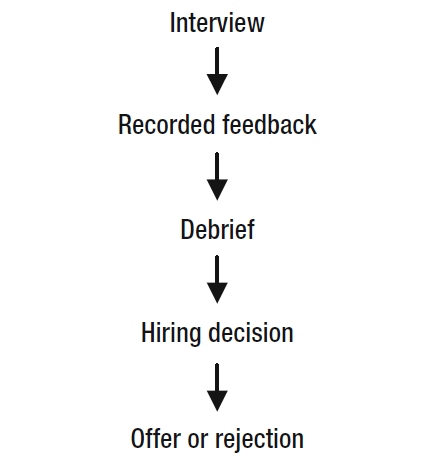
\includegraphics[width=6.1cm]{short_pipe}
  \caption{A short, straightforward evaluation pipe \cite[p.~42]{mcculler:book}.}
  \label{fig:short-pipe}
\end{figure}

It is important to have accurate and thorough understanding of a company and it's team construct. The process pipeline should be build based on this knowledge. The following Figure \vref{fig:typical-pipe} is an example of a typical high-level candidate pipeline from the hiring company's point of view.

\begin{figure}[h]
  \centering
  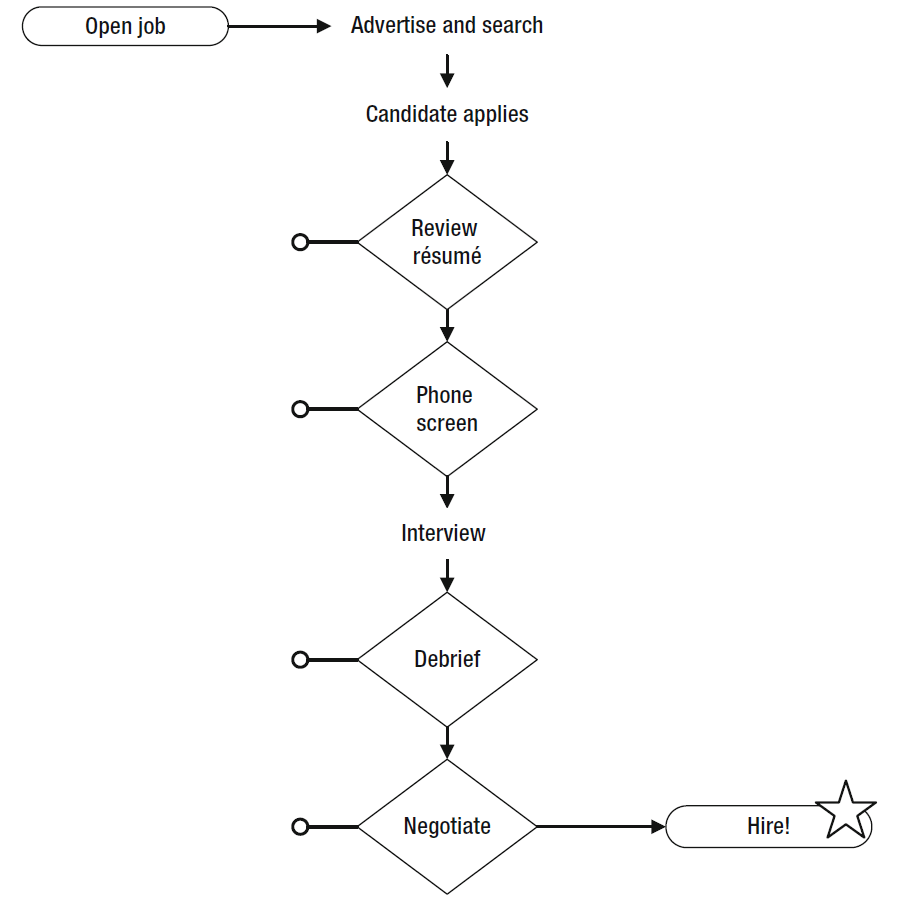
\includegraphics[width=12.2cm]{typical_pipe}
  \caption{An example of a high-level candidate pipeline \cite[p.~28]{mcculler:book}.}
  \label{fig:typical-pipe}
\end{figure}

In programming job openings it is sometimes beneficial to turn the evaluation process upside down, for example by starting with a code test and then interviewing the candidates that did well in the test. Also leaving the application letter out is one option when trying to make applying for the job more candidate friendly. The lower the bar of applying the more applications in total. \cite{noora:conversation}

What candidates appreciate the most is that the job advertisement is clear and the evaluation process is as transparent as possible so that the candidates are aware of their situation. Receiving feedback is also valued highly. \textbf{(aTalent rekrytointitutkimus 2014)} % cite will be from aTalent recruiting study from year 2014

Candidate always has the least knowledge about the company's pipeline and therefore informing them about what steps there are is a way to prevent misunderstandings \cite[p.~26]{mcculler:book}. The following Figure \vref{fig:candidate-pipe} is an example of what a typical pipeline from candidate's perspective looks like.

\begin{figure}[h]
  \centering
  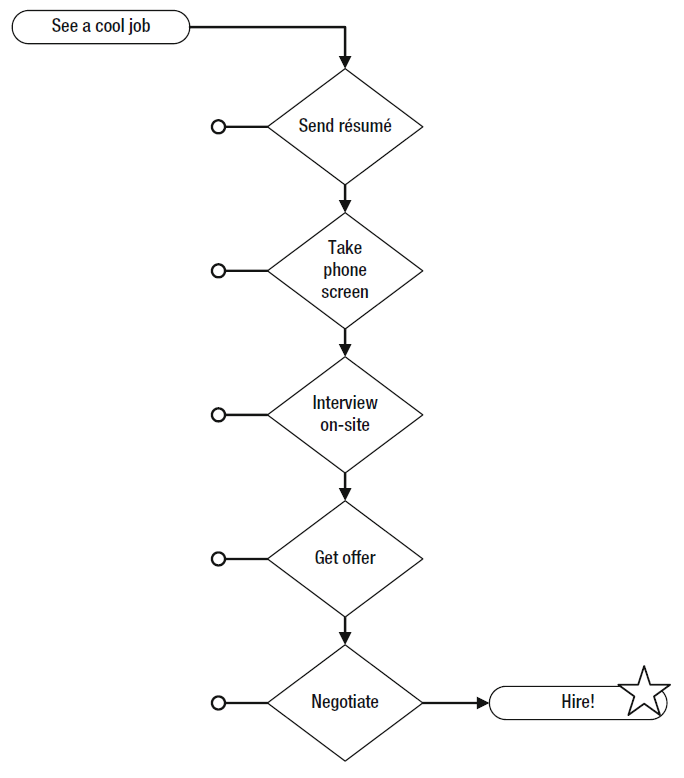
\includegraphics[width=10.8cm]{candidate_pipe}
  \caption{A candidate's perspective on their lifecycle in a typical pipeline \cite[p.~27]{mcculler:book}.}
  \label{fig:candidate-pipe}
\end{figure}

\subsection{Finding of suitable candidates}
\textbf{EXPLANATION:} Reading into clients’ minds and trying to find the key attributes and what is really required/wanted and what is just a bonus. 

%-------------------------------------------------------------------------------------
% JOKU HyVÄ ALKU TÄHÄN NÄIN
%-------------------------------------------------------------------------------------

When searching for and contacting candidates activity is the key. When a potential candidate turns up the recruiter should immediately try contacting them directly so as to be ahead of competitors. Most of the times recruiters are not going to get a direct response to their emails and a response rate of 20\% can be considered very good. When recruiters are contacting suitable employees they "are planting seeds, not everyone is going to respond to you right away." this means that companies contacting them will be remembered and that persistence will eventually lead to results. \textbf{(LÄHDE Ardy Daie)}

There are multiple different kinds of candidates but to summarize, a candidate is someone who "... may be actively looking for a job, passively looking, not looking but open to moving, not looking and actually quite content, or looking for a future position (such as after graduation)." \cite[p.~24]{mcculler:book} therefore using a combination of channels such as headhunting and job advertisements is the optimal way of reaching as many potential candidates as possible. The more channels available the better candidates usually can be found but if the job opening or the company is not appealing then it is best to strip the channels to a certain level to save resources.

Posting the job advertisement to company's website is the cheapest available channel while headhunting is generally the most expensive option. If the company is not well known and the amount of visitors in the company's website is low then the use of recruiting companies is also a valid option. The main benefits of using recruiting companies is that they have existing databases containing candidates as well as widespread connections such as with job boards, unions and subject associations to name a few. The price of recruiting companies varies but a single job advert to a job board can be hundreds of euros. \textbf{(MONSTER http://hiring.monster.com/recruitment/Standard-Postings.aspx)}

\subsection{Methods of evaluation}
\textbf{EXPLANATION:} How well candidates fit into role, what needs to be taken into consideration.

Content

\subsection{IT Recruiters' requirements}
\textbf{EXPLANATION:} What makes IT recruiting so difficult and how the recruiters can improve themselves / be educated to be enabled to do their work more efficiently and properly, what requirements need to be filled so that IT recruiter will excel in their work.

Knowledge of technologies
- Being interested in the industry
- Knowing at least the basics
- Overall knowledge of system architectures (what is backend, front end, what language is used where, what is full stack etc.)
- Knows the trends and what is in
The capability of finding stuff out
- activity
Standing against the challenges
Being good at finding what are the skills even if the candidate is socially awkward
What other things:
- Studies
    - University students are usually more competent
    - UAS students etc. the hobbyism and other projects are most important
- Can explain what they have done -> the more understandable and accurate the previous knowledge and job descriptions then usually the better the candidate
- \textbf{Application letter is sometimes irrelevant in IT recruiting}
- Diverse approaching methods
   - Sometimes the standard evaluation pipe is bad
   - Turning the process around -> First the test then interview
- Being quick and having discretion



\section{Defining candidate's skills}
\textbf{EXPLANATION:} Define skill so it can be referred later. Explain the concept of skill and some theoretical meters for skill comparisons.

There are people that are naturally very good at something. This might be misinterpreted as being skilled: "A skill is \textbf{a learned ability} to carry out a task with pre-determined results often within a given amount of time, energy, or both. In other words the abilities that one possesses. Skills can often be divided into domain-general and domain-specific skills." \cite[p. ~4]{howland:book}.

All skills must be obtained via practise. When someone has a biological prowess to learning something easily, such as mathematics or languages, they are not actually skilled in learning that thing, they are talented. When speaking of skilled learning then a person is using an array of tools and methods that make learning easier for them.

As previously cited most skills can be categorized into either of the two, domain-general or domain-specific skills. Domain-general skills are skills that could be used in more than a single task. These are much broader and a good example of such a skill could be social skills. Modern teaching theories emphasize, that instead of teaching dividual subjects it would be much better to try to build a bridge between them and merge them into a larger context \cite{mansoor:article}. A good concrete example of this are subjects like mathematics and physics, both of these thrive to explain how the world works and they both complement one another. There are some differences but knowing physics definitely does not affect mathematical competence. The reason why domain-general knowledge is often appreciated more is that when skills get combined into a larger context of knowledge and those skills actually become a tool that can be used to adapt to a vary of situations.

Most job descriptions require both domain-general and -specific skills, but there are also those that do not. Carpenters for instance can excel in their job without having many other skills outside of their carving skills. Or to modernize the job description there are companies that are looking for Java programmers for positions that only have a single requirement, being good at Java. When looking into a typical job description it is construct with skills from both categories of skill.

Skill can be measured. If a set of job applicants are provided with a region neutral test and all applicants are working under circumstances that are most favorable for their performance then the applicant with the most skill on the subject of the test should score the highest or if multiple candidates score the same highest score then finish the test the fastest. 

Situation like this is not very likely to happen however, for all the candidates to be at their best performance is very unlikely. Therefore measuring skill legitimately with any a test is actually incredibly difficult if there is any type of pressure involved such as in a situation where the test would be a delimiting factor for being hired or not. What companies can use such a test for is just as an addition to the whole recruitment process.

\subsection{Defining programming skills}
\textbf{EXPLANATION:} What is programming skill and what it consists of (logical thinking, algorithms, is it all math or does creativity have a place in it etc.).

Before trying to map out what are the things that programming skills could potentially consists of, it is necessary to define a programmer. A programmer is someone who writes computer software. In this case a computer could be any machine that can interpret binary code. A programmer's skills consists of domain-general and domain-specific skills. One of such a domain-specific skill is programming skills. These are "the skills required to write a program so that data may be processed by a computer" \cite{collins:skills}.  

In the list below there are some criteria that make a good programmer:
\vspace{-17pt} 
\begin{itemize}
\item Good knowledge of at least one programming language
\item Understanding of the underlying systems
\item Effective use of command line tools
\item Ability to debug
\item Capable of testing the code
\item Interest in current trends and future technologies
\item Motivated to learn the new
\item Co-operative, good at such things as team work and communication
\item Obtains problem solving skills
\end{itemize}
\vspace{-17pt}

Items such as "Good knowledge of at least one programming language" and "Capable of testing the code" are examples of domain-specific skills that correlate to programming skill.

A similar kind of list for a person with good programming skills could be something like the following:

\textbf{Find some better list!}

\vspace{-17pt} 
\begin{itemize}
\item Writes working and efficient code that is readable
\item Uses algorithms effectively
\item Makes sure that the code is as secure and safe from cyber-attacks as possible
\item Can create and maintain large projects with smart directory solutions
\item Knows the theory and can apply it to needs
\end{itemize}
\vspace{-17pt}

There are many areas of programming that the previous list doesn't cover and to define good programming skills would require a whole another study. 

\subsection{Evaluating the suitability of a candidate}
\label{sec:evaluating}
\textbf{EXPLANATION:} How to separate good programmers from bad and are there some global knowledge behind programming or is it all language specific etc. %PA: I don't very like "good or bad" there are usually shades of grey in-between... try to find more neutral terms? %JJ: Just an explanation for the chapter. See my comment on line 517

\textbf{EXPLANATION:} Also Existing platforms, methods etc.

When companies are trying to find the most suitable candidate for a job opening they will need to pinpoint the important attributes and skills that they are looking for and then execute a plan for evaluating applicants. One way of approach is to make a list containing both domain-general and domain-specific skills and use it in the initial elimination process and later as a tool for grading candidates and finding the most suitable one.

The following is a list of requirements that one Finnish company, specialized in providing integrated retail and supply chain planning solutions, used in one of their System and Network Administrator job openings: \cite{relex:apply}\newline
\textbf{In this role your responsibilities will include:}
\vspace{-17pt} 
\begin{itemize}
\item Deploy, maintain, configure, upgrade and retire servers and applications in accordance with company standards.
\item Manage firewalls and network devices.
\item Continually monitor network and server status using monitoring systems and react upon alarms.
\item Troubleshoot applications and system problems.
\item Participate in IT infrastructure development projects to support day to day operations and projects; investigate new technologies.
\end{itemize}
\vspace{-17pt}

\textbf{We value the following skills in our ideal candidates:}
\vspace{-17pt} 
\begin{itemize}
\item Prior professional experience of Linux System Administration
\item Prior experience with infrastructure hardware management and troubleshooting.
\item You master scripting (Bash, Python, etc.)
\item You are not afraid of responsibility and can handle multitasking
\item You are fluent in both verbal and written English
\item You have a good attitude, and you are fun to work with!
\end{itemize}
\vspace{-17pt}

\textbf{We consider as an advantage:}
\vspace{-17pt} 
\begin{itemize}
\item Knowledge of orchestration tools like Ansible or Docker
\item Experience with AWS or monitoring systems administration is also seen as an advantage
\item Fluency in Finnish, Swedish, German, French or Italian
\end{itemize}
\vspace{-17pt}

\textbf{(TÄTÄ SEURAAVAA OSIOTA VOIS PARANTAA)}

In the previous example the first section consists of the big themes and is useful when the recruiter has found multiple suitable candidates and differentiating has become difficult. The second section is what is used to do most of the eliminating consisting of both domain-general and -specific skills. Time periods such as "prior experience" are used to secure that candidates have the competence to manage those areas of the job. There are some attributes on the list that have to do with ones capability-tools and in many cases those are weighted as most valuable. Last section consists of domain-specific skills that can be used to make separations between otherwise equally capable candidates.

\textbf{(Sori hanna myös tää seuraava osio on aika kauhee)}

After the applying deadline has passed, if there is any, and the basic screening has been done and all candidates' portfolio, CV and application letter has been reviewed and the recruiter has come to a conclusion to whom should be proceeding in the recruitment process it is good to inform all candidates whether they have been approved to move onwards in the recruitment process or declined. It is important for \gls{eb} that all applicants are informed since treating candidates as customers results in making the general view of the company more positive and the declined candidates will more likely apply for other positions that may open in the future.

If the recruiting company is uncertain of how advanced the candidates are in programming there is always the option of using a code test or multiple tests. Coding tests are becoming a crucial part of the IT recruiting process, because when build right they can give quick and accurate information about the global knowledge of the candidate \cite{winter:blog}. There are a few approaches to code tests but to build a language neutral code test, a test that is not specifically for a certain programming language and can be used in several job openings, the use of pseudo code, a language that is often used when teaching the basics of thinking as a programmer, is recommended due to it's nature of not favouring anyone.

\textbf{EXPLANATION:} Existing platforms, methods etc.

There are also some companies that are specialized in code test platforms that are easy to use, sometimes even containing existing code tests to choose from. Some of these platforms are very advanced providing real time screen sharing, direct contacting and advanced tools for ranking the candidates. The price tag on these platforms is usually quite high, for instance Codility's cheapest model costs \$159/month and is limited to just fifteen test attempts \cite{codility}. Companies that are recruiting on frequent basis but do not have a lot of capital the more realistic option is using some platform that simply uses multiple choice questions instead, an example of such a platform is ProProfs\cite{proprofs}.



\textbf{Figure tähän}



\subsection{Other ways of information gathering}
\textbf{EXPLANATION:} Looking into the applicant’s profile and skillset (LinkedIn, GH, SO, Education, Motivation (Letter / CV), recommendations, hobbyism).
\chapter{Methods and materials}
\textbf{EXPLANATION:} How was the project carried out in practise, and how was the data analysed? Describe the context in which the work was carried out (such as the overall project and its desing, your specific task, work environment) and the workflow. Describe the methods and materials used (accurate details of data, software, materials, methods, techniques). Give a full account of exact test arrangements and measurements carried out, and accurate details of data analysis. The issues included in this section depend on the nature of your project. Whatever the issues, describe them in sufficient detail and in logical sequence.

According to Fenton and Pfleeger \cite{fenton_pfleeger:book} the mathematical definition of a metric is "a rule
used to describe how far apart two point are. More formally, a metric is a function m defined
on pairs of objects x and y such that m(x,y) represents the distance between x and y".

\section{Using code tests as a way of evaluation}
\section{Ways of mitigating and simplifying the IT recruitment process}
\textbf{EXPLANATION:} Going through all the problematic parts explained in the theoretical part of the thesis and grabbing a single subject that could potentially be improved.

\subsection{Programmatic solutions to recruitment process problems}
\textbf{EXPLANATION:} What could be improved via programming, screen some options and select one of them. Explaining why the specific subject was chosen and introduce what existing data such as APIs (GH and SO) could be used.

\subsection{Building of an applicant compatibility evaluator}
\textbf{EXPLANATION:} Dig in deeper to APIs and the algorithms behind the evaluator. Also what thoughts and how well did the application fill its’ role (was it useful/not why?).
\chapter{Results}
\textbf{EXPLANATION:} What was found/created/designed/produced? This section should include a clear presentation of the results, even possible errors and sources of errors. Use an appropriate mixture of text, tables and figures. In this section you should also say if you met the goal(s) set in the introduction.
\chapter{Discussion}
\textbf{EXPLANATION:} What do the results mean? Evaluate the results and the project: such as benefits and drawbacks, reliability, significance and usefulness of the results, validity of any conclusions drawn from the results, technical and economical aspects. Discuss, for example, possibilities of applying the results for other purposes than the initial, and problems encountered during the project and decisions made. Evaluate whatever the goal set in the introduction was met: compare the results with those expected. Provide a critical and objectibe ebaluation of the results and implementation of your project, and place the results in context with previous studies (discussed in the theoretical background section).
\chapter{Conclusion}
\textbf{EXPLANATION:} What can be concluded? This section usually begins with a restatement of the goal of the project, and includes a brief summary of the key results of the project and a conclusion about the significance and implications of the results, for your client ant perhaps the field in general. Also mention strengths and limitations of the project and ways in which the project could be changed and improved if carried out again. In the end recommend further action, such as further study, if relevant. Keep this section short (a few paragraphs, no subheadings), tie in and highlight the main points of the project and its results and draw a clear conclusion.



\section{}
Here is an example how to add biblio entry \cite{kopka:guide} using the \textquotedblleft\textbackslash{}cite\textquotedblright ~\gls{latex} command ~\cite[section 4.2]{tobias:book}. Note that a paragraph is added by forcing a new line.

And let also try the figure (see figure \vref{fig:latex-cover}) and internal reference (with label and ref or vref). The reference can be done to any label, for example why not to appendix \ref{appx:first} or to appendix \ref{appx:second}? To note, \gls{latex} will place the figure to the best place (except with forcing). Let them float till the final of final edit\ldots ~then force them to not break a paragraph.%hugly hack... I'm sorry
\begin{figure}[h]
  \centering
  
\includegraphics[width=7.1cm]{LaTeX_cover}
  \caption{\gls{latex} cover image (Copied from wikibooks.org (2012) \cite{wikibooks:latex}).}
  \label{fig:latex-cover}
\end{figure}

Let's also try a long quote:
From the Universal Declaration of Human Rights:
\begin{quote}
(1) Everyone has the right to education. Education shall be free, at least in the elementary and fundamental stages. Elementary education shall be compulsory. Technical and professional education shall be made generally available and higher education shall be equally accessible to all on the basis of merit.

(2) Education shall be directed to the full development of the human personality and to the strengthening of respect for human rights and fundamental freedoms. It shall promote understanding, tolerance and friendship among all nations, racial or religious groups, and shall further the activities of the United Nations for the maintenance of peace.

(3) Parents have a prior right to choose the kind of education that shall be given to their children. \cite[article 26]{un:udhr}
\end{quote}

\textit{Quisque augue} est, \textbf{elementum ac porttitor} non, porttitor ac orci. Donec hendrerit, ligula ac luctus egestas, sem dolor pretium nunc, sed vehicula magna diam a massa. Donec mattis, arcu et tempor mattis, risus tortor ultrices metus, nec sodales sem dolor eu elit.\vspace{-17pt} 
\begin{itemize}
\item \textbf{A small hack} with list
\item is to force the vertical space 
\item before and after the list
\end{itemize}
\vspace{-17pt} Nullam egestas enim at odio pellentesque bibendum. 

\subsection{Subsection}
Donec et sapien ac leo condimentum vulputate id et tellus. Maecenas hendrerit malesuada interdum. Aenean dignissim sem faucibus elit congue faucibus id non risus. Morbi at dui non tortor pellentesque consequat non eget urna. Cras in sapien dui, a tincidunt velit.
\reaction{\label{eq:reaktio}$\underset{\text{+II}}{\ce{2Fe^2+}}$ + $\underset{\text{+I\;-I}}{\ce{H2O2}}$ + $\underset{\text{+I\;-II}}{\ce{2H3O^+}}$ <=> $\underset{\text{+III}}{\ce{2Fe^3+}}$ + $\underset{\text{+I\;-II}}{\ce{4H2O}}$}
Työn aluksi rauta(II)ionit hapetetaan rauta(III)ioneiksi väkevällä vetyperoksidilla, kuten reaktion~\ref{eq:reaktio} hapetusluvuista nähdään (rauta hapettuu, happi pelkistyy).  
\reaction{Fe^3+( \emph{aq} ) + 3OH^-( \emph{aq} ) + $(x-1)$H2O( \emph{l} ) -> FeOOH $\cdot$ $x$(H2O)( \emph{s} )}
Rauta(III)ionit saostetaan emäksen (\ce{NH3}) avulla ja saadaan tuotteeksi kidevedellinen rauta(III)hydroksidi. Saatu saostuma pestään \ce{NH4NO3}:lla.
\reaction{FeOOH $\cdot$ $x$(H2O)( \emph{s} ) ->T[$\Delta$900-1000\celsius] Fe2O3( \emph{s} )}

\subsection{Subsection with \Gls{maths}}
Donec et sapien ac leo condimentum vulputate id et tellus. Maecenas hendrerit malesuada interdum. Aenean dignissim sem faucibus elit congue faucibus id non risus. Morbi at dui non tortor pellentesque consequat non eget urna. Cras in sapien dui, a tincidunt velit. Tertiäärinen butyylikloridi reagoi veden kanssa oheisen reaktion mukaisesti:
\reaction{(CH3)3CCl + 2H2O -> (CH3)3COH+H3O+ +Cl-}
Kyseessä on ensimmäisen kertaluvun reaktio, joten reaktion nopeus on
\begin{align}
v=-\frac{\mathrm{d}[\tn{t-ButCl}]}{\mathrm{d}t}=\frac{\mathrm{d}[\tn{HCl}]}{\mathrm{d}t}=k[\tn{t-ButCl}]
\end{align}
Jos tarkastellaan lähtöaineen t-butyylikloridin häviämistä saadaan
\begin{align}
\frac{\mathrm{d}[\tn{t-ButCl}]}{[\tn{t-ButCl}]}&=-k\mathrm{d}t \\
\int \frac{\mathrm{d}[\tn{t-ButCl}]}{[\tn{t-ButCl}]}&=-k \int \mathrm{d}t \\
\ln \int_{[\tn{t-ButCl}]_0}^{[\tn{t-ButCl}]} [\tn{t-ButCl}]&=-k\int_0^t t \\
\ln \left( \frac{[\tn{t-ButCl}]}{[\tn{t-ButCl}]_0} \right)&=-kt
\end{align}
Ionivahvuus lasketaan kaavalla.
\begin{align}
I&=\frac{1}{2}\cdot\sum z_i^2c_i \\
z_i&= \tn{ionin varausluku} \\
c_i&= \tn{ionin konsentraatio}
\end{align}
Aktiivisuuskerroin $\gamma_\pm$ lasketaan kaavalla.
\begin{align}
\log \gamma_\pm &= -\left|z_+\cdot z_-\right|A\cdot I^{\frac{1}{2}} \\
A &= \tn{0,509 (lämpötilassa 25\celsius}) \\
I &= \tn{ionivahvuus} \\
z &= \tn{ionien varaus}
\end{align}

\section{Section with Source Code}
Donec et sapien ac leo condimentum vulputate id et tellus. Maecenas hendrerit malesuada interdum. Aenean dignissim sem faucibus elit congue faucibus id non risus. Morbi at dui non tortor pellentesque consequat non eget urna. Cras in sapien dui, a tincidunt velit.

\begin{lstlisting}[language=PHP,caption={Descriptive Caption Text},label=testphp] 
<?php
$userName = $_POST["usern"];
//maybe not?
if ($userName){
	?>
	<h2>Hello <?php echo $userName; ?>!</h2>
	<p>your message got received.</p>
	<?php
}
?>
\end{lstlisting}\vspace{-17pt}


As see in listing \ref{testphp}: Donec et sapien ac leo condimentum vulputate id et tellus. Maecenas hendrerit malesuada interdum. Aenean dignissim sem faucibus elit congue faucibus id non risus. Morbi at dui non tortor pellentesque consequat non eget urna. Cras in sapien dui, a tincidunt velit.

\section{Section with Table}
Donec et sapien ac leo condimentum vulputate id et tellus. Maecenas hendrerit malesuada interdum. Aenean dignissim sem faucibus elit congue faucibus id non risus. Morbi at dui non tortor pellentesque consequat non eget urna. Cras in sapien dui, a tincidunt velit.

\begin{table}[h]
  \centering
  \caption{Some data}
  %IMPORTANT the caption must be before the tabular, so it will be on top of the table (there are other tricks to force it on top; but this one is straitforward).
  \begin{tabular}{| l | >{\centering\arraybackslash}p{.5\textwidth} |}
    \hline
    Test 1 & test 1234 test \\
    \hline
    Some more date comes here & with more values and if the text is very long it will disappear out of the box unless you force the column size :( \\
    \hline
  \end{tabular}
  \label{table:some_data}
\end{table}


As presented in table \ref{table:some_data}: Donec et sapien ac leo condimentum vulputate id et tellus. Maecenas hendrerit malesuada interdum. Aenean dignissim sem faucibus elit congue faucibus id non risus. Morbi at dui non tortor pellentesque consequat non eget urna. Cras in sapien dui, a tincidunt velit.

\begin{table}[h]
  \centering
  \caption{Another table with tabularx}
  \begin{tabularx}{.95\textwidth}{| l | >{\centering\arraybackslash} X |}
    \hline
    Test 1 & test 1234 test \\
    \hline
    Some more date comes here & with more values and if the text is very long it will disappear out of the box unless you force the table size :( \\
    \hline
  \end{tabularx}
  \label{table:some_data2}
\end{table}

As presented in table \ref{table:some_data2}: Donec et sapien ac leo condimentum vulputate id et tellus. Maecenas hendrerit malesuada interdum. Aenean dignissim sem faucibus elit congue faucibus id non risus. Morbi at dui non tortor pellentesque consequat non eget urna. Cras in sapien dui, a tincidunt velit.

\begin{table}[htbp]
  \centering
  \caption{Booktabs example}
    \begin{tabular}{rrrr}
    \toprule
    t (s) & [HCl] & [t-ButCl] & $\ln\frac{[t-ButCl]}{[t-ButCl]_0}$ \\
    \midrule
    0     & 4,02  & 160,88 & 0,00 \\
    10    & 63    & 101,9 & -0,46 \\
    20    & 115,2 & 49,7  & -1,17 \\
    30    & 141,3 & 23,6  & -1,92 \\
    40    & 157,9 & 7     & -3,13 \\
    50    & 161   & 3,9   & -3,72 \\
    60    & 164,3 & 0,6   & -5,59 \\
    70    & 163,5 & 1,4   & -4,74 \\
    80    & 163,8 & 1,1   & -4,99 \\
    90    & 164,1 & 0,8   & -5,30 \\
    100   & 164,3 & 0,6   & -5,59 \\
    \bottomrule
    \end{tabular}
  \label{tab:thisislabel}
\end{table}

\chapter{Second Chapter}

Lorem ipsum dolor sit amet, consectetur adipiscing elit. Aliquam aliquam aliquam purus, in ornare nulla imperdiet molestie. Nam tempus erat eu dui rhoncus et vestibulum mi elementum. Ut porttitor elit sit amet justo dignissim sit amet sagittis massa egestas. Mauris sed dolor eget dui fermentum sodales ut eu nibh. 

Quisque augue est, elementum ac porttitor non, porttitor ac orci. Donec hendrerit, ligula ac luctus egestas, sem dolor pretium nunc, sed vehicula magna diam a massa. Donec mattis, arcu et tempor mattis, risus tortor ultrices metus, nec sodales sem dolor eu elit. Nullam egestas enim at odio pellentesque bibendum. 

Donec et sapien ac leo condimentum vulputate id et tellus. Maecenas hendrerit malesuada interdum. Aenean dignissim sem faucibus elit congue faucibus id non risus. Morbi at dui non tortor pellentesque consequat non eget urna. Cras in sapien dui, a tincidunt velit.

\chapter{Third Chapter}

Lorem ipsum dolor sit amet, consectetur adipiscing elit. Aliquam aliquam aliquam purus, in ornare nulla imperdiet molestie. Nam tempus erat eu dui rhoncus et vestibulum mi elementum. Ut porttitor elit sit amet justo dignissim sit amet sagittis massa egestas. Mauris sed dolor eget dui fermentum sodales ut eu nibh.
\begin{figure}[htbp]
  \centering
    \begin{tikzpicture}
        \pgfplotsset{width=12cm,
        compat=1.3,
        legend style={font=\footnotesize}}
    \begin{axis}[
    xlabel={c (mg/l)},
    ylabel={A},
    legend pos=north west,
    ymajorgrids=true,
    grid style=dashed
]

\addplot [only marks, blue] table {data.dat};
\addplot [no markers, thick, red] table[
x=c,
y={create col/linear regression}] {data.dat};
\addlegendentry{data}
\addlegendentry{%
$\pgfmathprintnumber{\pgfplotstableregressiona}x
\pgfmathprintnumber[print sign]{\pgfplotstableregressionb}$}
\end{axis}
\end{tikzpicture}
\label{fig:stdplot}
\caption{Simple linear regression plot (cannot get $r^2$ value)}
\end{figure}
Quisque augue est, elementum ac porttitor non, porttitor ac orci. Donec hendrerit, ligula ac luctus egestas, sem dolor pretium nunc, sed vehicula magna diam a massa. Donec mattis, arcu et tempor mattis, risus tortor ultrices metus, nec sodales sem dolor eu elit. Nullam egestas enim at odio pellentesque bibendum. 

Donec et sapien ac leo condimentum vulputate id et tellus. Maecenas hendrerit malesuada interdum. Aenean dignissim sem faucibus elit congue faucibus id non risus. Morbi at dui non tortor pellentesque consequat non eget urna. Cras in sapien dui, a tincidunt velit.

\section{Section}

Lorem ipsum dolor sit amet, consectetur adipiscing elit. Aliquam aliquam aliquam purus, in ornare nulla imperdiet molestie. Nam tempus erat eu dui rhoncus et vestibulum mi elementum. 
\tikzstyle{palikka} = [rectangle, rounded corners, minimum width=1cm, minimum height=1cm, text centered, text width=2cm, draw=black, fill=red!30]
\tikzstyle{arrow} = [thick,->,>=stealth]
\begin{figure}[htbp]
\centering
\begin{tikzpicture}[node distance=2.75cm]
\node[label=90:Label] (yksi) [palikka] {Lorem};
\node (kaksi) [palikka, right of=yksi] {ipsum};
\node (kolme) [palikka, below of=kaksi,  yshift=1cm] {dolor};
\node (neljä) [palikka, left of=kolme] {sit};
\node (viisi) [palikka, below of=neljä, yshift=1cm] {amet};
\draw [arrow] (yksi) -- (kaksi);
\draw [arrow] (kaksi) -- node[anchor=west] {tekstiä} (kolme);
\draw [arrow] (kolme) -- (neljä);
\draw [arrow] (neljä) -- (viisi);
\end{tikzpicture}
\caption{Example tikz-picture}
\label{fig:tikz}
\end{figure}
Ut porttitor elit sit amet justo dignissim sit amet sagittis massa egestas. Mauris sed dolor eget dui fermentum sodales ut eu nibh. 

\section{Section}

Lorem ipsum dolor sit amet, consectetur adipiscing elit. Aliquam aliquam aliquam purus, in ornare nulla imperdiet molestie. Nam tempus erat eu dui rhoncus et vestibulum mi elementum. Ut porttitor elit sit amet justo dignissim sit amet sagittis massa egestas. Mauris sed dolor eget dui fermentum sodales ut eu nibh. 

%----------------------------------------------------------------------------------------
%   BIBLIOGRAPHY 
%----------------------------------------------------------------------------------------

\IfLanguageName{finnish}{\bibliographystyle{vancouver_fi}}{\bibliographystyle{vancouver}}
%line space
%\singlespacing %removed otherwise the appendix are also single space
\begin{flushleft}
\begin{singlespacing}
\bibliography{biblio}
\end{singlespacing}
\end{flushleft}

%for conting the pages
\label{LastPage}~


%----------------------------------------------------------------------------------------
%   APPENDICES 
%----------------------------------------------------------------------------------------
%avoid that the last page of bib get appendix header
\clearpage
%start appendix
\appendix
%no page number for appendix in table of content
\addtocontents{toc}{\cftpagenumbersoff{chapter}}
%appendix sections and subsections not in table of content
\settocdepth{chapter}
%add "Appendices" in the table of content
\addappheadtotoc
%force smaller vertical spacing in table of content
%!!! There can be some fun depending if the appendices have (sub)sections or not :D
% You will have to play with these numbers and eventually copy the \pretocmd line on before some \chapter and force another number.
\addtocontents{toc}{\vspace{11pt}}
\pretocmd{\chapter}{\addtocontents{toc}{\protect\vspace{-24pt}}}{}{}
%have Appendix 1 (instead of Appendix A)
\renewcommand{\thechapter}{\arabic{chapter}} 

\newcommand\liite[1]{
%each appendix restart page num to one
\setcounter{page}{1}
%special counter for appendix TODO: this is a ugly quick hack :( Should find a better way to count the page per appendix.
\newtotcounter{appx#1}
%overwrite the header
\makeevenhead{plain}{}{}{\appname \thechapter \\ \thepage\,(\stepcounter{appx#1}\total{appx#1})}
\makeoddhead{plain}{}{}{\appname \thechapter \\ \thepage\,(\stepcounter{appx#1}\total{appx#1})}}

\liite{1}
\chapter{My First Appendix}\label{appx:first}

Note that every appendix will be a chapter.

Sorry for the ugly hack on how to count the total pages per appendix.


Of course with section and subsection.

\section{Appendix Section}

And you can cite \cite{tobias:book} stuff, it will go into the main bibliography.

Lorem ipsum dolor sit amet, consectetur adipiscing elit. Aliquam aliquam aliquam purus, in ornare nulla imperdiet molestie. Nam tempus erat eu dui rhoncus et vestibulum mi elementum. Ut porttitor elit sit amet justo dignissim sit amet sagittis massa egestas. Mauris sed dolor eget dui fermentum sodales ut eu nibh.

\subsection{With a Subsection}

Lorem ipsum dolor sit amet, consectetur adipiscing elit. Aliquam aliquam aliquam purus, in ornare nulla imperdiet molestie. Nam tempus erat eu dui rhoncus et vestibulum mi elementum. Ut porttitor elit sit amet justo dignissim sit amet sagittis massa egestas. Mauris sed dolor eget dui fermentum sodales ut eu nibh.

Quisque augue est, elementum ac porttitor non, porttitor ac orci. Donec hendrerit, ligula ac luctus egestas, sem dolor pretium nunc, sed vehicula magna diam a massa. Donec mattis, arcu et tempor mattis, risus tortor ultrices metus, nec sodales sem dolor eu elit. Nullam egestas enim at odio pellentesque bibendum. 

Donec et sapien ac leo condimentum vulputate id et tellus. Maecenas hendrerit malesuada interdum. Aenean dignissim sem faucibus elit congue faucibus id non risus. Morbi at dui non tortor pellentesque consequat non eget urna. Cras in sapien dui, a tincidunt velit.

\clearpage % avoid that the last page of previous appendix get this header
\liite{2}
\chapter{My Second Appendix}\label{appx:second}
\addtocontents{toc}{\vspace{11pt}}

Lorem ipsum dolor sit amet, consectetur adipiscing elit. Aliquam aliquam aliquam purus, in ornare nulla imperdiet molestie. Nam tempus erat eu dui rhoncus et vestibulum mi elementum. Ut porttitor elit sit amet justo dignissim sit amet sagittis massa egestas. Mauris sed dolor eget dui fermentum sodales ut eu nibh.

Quisque augue est, elementum ac porttitor non, porttitor ac orci. Donec hendrerit, ligula ac luctus egestas, sem dolor pretium nunc, sed vehicula magna diam a massa. Donec mattis, arcu et tempor mattis, risus tortor ultrices metus, nec sodales sem dolor eu elit. Nullam egestas enim at odio pellentesque bibendum. 

\clearpage
\liite{3}
\chapter{R examples}
TODO
\end{document}
